% (find-LATEX "2020-1-C3-miniteste-2.tex")
% (defun c () (interactive) (find-LATEXsh "lualatex -record 2020-1-C3-miniteste-2.tex" :end))
% (defun D () (interactive) (find-pdf-page      "~/LATEX/2020-1-C3-miniteste-2.pdf"))
% (defun d () (interactive) (find-pdftools-page "~/LATEX/2020-1-C3-miniteste-2.pdf"))
% (defun e () (interactive) (find-LATEX "2020-1-C3-miniteste-2.tex"))
% (defun u () (interactive) (find-latex-upload-links "2020-1-C3-miniteste-2"))
% (defun v () (interactive) (find-2a '(e) '(d)) (g))
% (find-pdf-page   "~/LATEX/2020-1-C3-miniteste-2.pdf")
% (find-sh0 "cp -v  ~/LATEX/2020-1-C3-miniteste-2.pdf /tmp/")
% (find-sh0 "cp -v  ~/LATEX/2020-1-C3-miniteste-2.pdf /tmp/pen/")
%   file:///home/edrx/LATEX/2020-1-C3-miniteste-2.pdf
%               file:///tmp/2020-1-C3-miniteste-2.pdf
%           file:///tmp/pen/2020-1-C3-miniteste-2.pdf
% http://angg.twu.net/LATEX/2020-1-C3-miniteste-2.pdf
% (find-LATEX "2019.mk")

% «.regras»	(to "regras")
% «.scans»	(to "scans")

\documentclass[oneside,12pt]{article}
\usepackage[colorlinks,citecolor=DarkRed,urlcolor=DarkRed]{hyperref} % (find-es "tex" "hyperref")
\usepackage{amsmath}
\usepackage{amsfonts}
\usepackage{amssymb}
\usepackage{pict2e}
\usepackage[x11names,svgnames]{xcolor} % (find-es "tex" "xcolor")
%\usepackage{colorweb}                 % (find-es "tex" "colorweb")
%\usepackage{tikz}
%
% (find-dn6 "preamble6.lua" "preamble0")
%\usepackage{proof}   % For derivation trees ("%:" lines)
%\input diagxy        % For 2D diagrams ("%D" lines)
%\xyoption{curve}     % For the ".curve=" feature in 2D diagrams
%
\usepackage{edrx15}               % (find-LATEX "edrx15.sty")
\input edrxaccents.tex            % (find-LATEX "edrxaccents.tex")
\input edrxchars.tex              % (find-LATEX "edrxchars.tex")
\input edrxheadfoot.tex           % (find-LATEX "edrxheadfoot.tex")
\input edrxgac2.tex               % (find-LATEX "edrxgac2.tex")
%
%\usepackage[backend=biber,
%   style=alphabetic]{biblatex}            % (find-es "tex" "biber")
%\addbibresource{catsem-slides.bib}        % (find-LATEX "catsem-slides.bib")
%
% (find-es "tex" "geometry")
\usepackage[a6paper, landscape,
            top=1.5cm, bottom=.25cm, left=1cm, right=1cm, includefoot
           ]{geometry}
%
\begin{document}

\catcode`\^^J=10
\directlua{dofile "dednat6load.lua"}  % (find-LATEX "dednat6load.lua")

% «defs»  (to ".defs")
% (find-LATEX "edrx15.sty" "colors-2019")
\long\def\ColorRed   #1{{\color{Red1}#1}}
\long\def\ColorViolet#1{{\color{MagentaVioletLight}#1}}
\long\def\ColorViolet#1{{\color{Violet!50!black}#1}}
\long\def\ColorGreen #1{{\color{SpringDarkHard}#1}}
\long\def\ColorGreen #1{{\color{SpringGreenDark}#1}}
\long\def\ColorGreen #1{{\color{SpringGreen4}#1}}
\long\def\ColorGray  #1{{\color{GrayLight}#1}}
\long\def\ColorGray  #1{{\color{black!30!white}#1}}
\long\def\ColorBrown #1{{\color{Brown}#1}}
\long\def\ColorBrown #1{{\color{brown}#1}}

\long\def\ColorShort #1{{\color{SpringGreen4}#1}}
\long\def\ColorLong  #1{{\color{Red1}#1}}

\def\frown{\ensuremath{{=}{(}}}
\def\True {\mathbf{V}}
\def\False{\mathbf{F}}

\def\drafturl{http://angg.twu.net/LATEX/2020-1-C2.pdf}
\def\drafturl{http://angg.twu.net/2020.1-C2.html}
\def\draftfooter{\tiny \href{\drafturl}{\jobname{}} \ColorBrown{\shorttoday{} \hours}}


%  _____ _ _   _                               
% |_   _(_) |_| | ___   _ __   __ _  __ _  ___ 
%   | | | | __| |/ _ \ | '_ \ / _` |/ _` |/ _ \
%   | | | | |_| |  __/ | |_) | (_| | (_| |  __/
%   |_| |_|\__|_|\___| | .__/ \__,_|\__, |\___|
%                      |_|          |___/      
%
% «title»  (to ".title")
% (c3m201mt2p 1 "title")
% (c3m201mt2    "title")

\thispagestyle{empty}

\begin{center}

\vspace*{1.2cm}

{\bf \Large Cálculo 3 - 2020.1}

\bsk

Mini-teste 2

\bsk

Eduardo Ochs - RCN/PURO/UFF

\url{http://angg.twu.net/2020.1-C3.html}

\end{center}

%\printbibliography

\newpage

%  ____                          
% |  _ \ ___  __ _ _ __ __ _ ___ 
% | |_) / _ \/ _` | '__/ _` / __|
% |  _ <  __/ (_| | | | (_| \__ \
% |_| \_\___|\__, |_|  \__,_|___/
%            |___/               
%
% «regras»  (to ".regras")
% (c3m201mt2p 2 "regras")
% (c3m201mt2    "regras")

% (c3m201pltanp 11 "mini-teste-1")
% (c3m201pltan     "mini-teste-1")
% (c3m201pltanp 12 "miniteste-regras")
% (c3m201pltan     "miniteste-regras")
% (c2m201mt1p 7 "miniteste-regras")
% (c2m201mt1    "miniteste-regras")

{\bf Regras:}

As questões do mini-teste foram disponibilizadas na quarta-feira
25/nov/2020, às 19:05 por JPG no Telegram e às 20:15 por este PDF.
Você deverá entregar as respostas \ColorRed{escritas à mão} até as
20:15 da quinta-feira 26/nov/2020 na plataforma Classroom. Se o
Classroom der algum problema mande também para este endereço de
e-mail:

\ssk

\ColorRed{eduardoochs@gmail.com}

\ssk

Mini-testes entregues após este horário não serão considerados.

Durante as 24 horas do mini-teste nem o professor nem o monitor
responderão perguntas sobre os assuntos do mini-teste \ColorRed{mas
  você pode discutir com os seus colegas --- inclusive no grupo da
  turma.}

% , mas não durante o horário da aula.

Este mini-teste vale 0.5 pontos extras na P1.

\newpage

{\bf Regras (cont.):}

\ssk

Os alunos que cumprirem uma série de condições (ainda não divulguei a
lista delas...) poderão compensar as suas questões erradas na P2
fazendo vídeos explicando passo a passo como resolvê-las na semana
seguinte à prova. \ColorRed{Uma das condições é ter feito todos os
  mini-testes, então não deixe de fazer e entregar este mini-teste!}

\bsk
\bsk

{\bf Regra importantíssima, que vale só para este mini-teste:}

{\bf Contas fora do ponto base zeram a questão!!!}



\newpage

% (find-latexscan-links "C3" "20201125_C3_mt2")
% (find-xpdf-page "~/LATEX/2020-1-C3/20201125_C3_mt2.pdf")
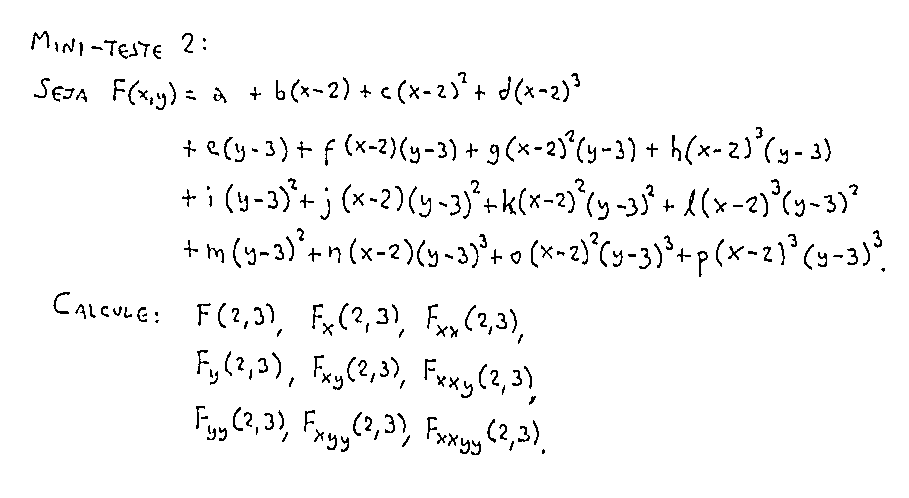
\includegraphics[width=12cm]{2020-1-C3/20201125_C3_mt2.pdf}


\newpage

\def\x   {(x-x_0)}
\def\xx  {(x-x_0)^2}
\def\xxx {(x-x_0)^3}
\def\xxxx{(x-x_0)^4}
\def\y   {(y-y_0)}
\def\yy  {(y-y_0)^2}
\def\yyy {(y-y_0)^3}
\def\yyyy{(y-y_0)^4}

Correção: é

$\scalebox{0.75}{$
 \begin{array}{rcllllllll}
 F(x,y)&=& a      &+ b \x      &+ c \xx      &+ d \xxx      \\
       &+& e \y   &+ f \x \y   &+ g \xx \y   &+ h \xxx \y   \\
       &+& i \yy  &+ j \x \yy  &+ k \xx \yy  &+ l \xxx \yy  \\
       &+& m \yyy &+ n \x \yyy &+ o \xx \yyy &+ p \xxx \yyy \\
 \end{array}
 $}
$


\end{document}

% «scans»  (to ".scans")
% (find-LATEX "2020-1-C3-aprox-2a-ordem-R2.tex" "scans")
# (find-LATEX "2020-1-C2-subst-trig-1.tex" "scans")

 (eepitch-shell)
 (eepitch-kill)
 (eepitch-shell)
# (find-fline "~/2020.1-C3/")
# (find-fline "/tmp/qc3/")
# (find-fline "/tmp/")
# (find-fline "/tmp/c3mt2/")
# (find-fline "~/LATEX/2020-1-C3/")
cd /tmp/qc3/
cd /tmp/
f () { rm -fv $1.png $1.pdf; djvuize $1.pdf }
f () { rm -fv $1.png $1.pdf; djvuize WHITEBOARDOPTS="-m 0.5" $1.pdf; xpdf $1.pdf }
f () { rm -fv $1.png $1.pdf; djvuize WHITEBOARDOPTS="-m 0.25" $1.pdf; xpdf $1.pdf }
f () { cp -fv $1.png $1.pdf       ~/2020.1-C3/ }
f () { cp -fv        $1.pdf ~/LATEX/2020-1-C3/ }
f () { cp -fv $1.png $1.pdf       ~/2020.1-C3/
       cp -fv        $1.pdf ~/LATEX/2020-1-C3/
     }
f () { echo "% (find-latexscan-links \"C3\" \"$1\")" }

f 20201125_C3_mt2



%  __  __       _        
% |  \/  | __ _| | _____ 
% | |\/| |/ _` | |/ / _ \
% | |  | | (_| |   <  __/
% |_|  |_|\__,_|_|\_\___|
%                        
% <make>

 (eepitch-shell)
 (eepitch-kill)
 (eepitch-shell)
# (find-LATEXfile "2019planar-has-1.mk")
make -f 2019.mk STEM=2020-1-C3-miniteste-2 veryclean
make -f 2019.mk STEM=2020-1-C3-miniteste-2 pdf

% Local Variables:
% coding: utf-8-unix
% ee-tla: "c3m201mt2"
% End:
